\section{Моделирование последовательностного подхода обнаружения аномалий}

Для демонстрации работоспособности подхода по обнаружению аномалий в Kubernetes-кластере использован публичный набор данных HDFS\_v1 из коллекции LogHub. Данный набор содержит более 11 миллионов лог-записей, сгруппированных по идентификатору блока, и включает разметку нормальных и аномальных трасс выполнения системы \cite{HDFS_dataset}.

В рамках эксперимента рассматривается применение последовательностного подхода к анализу лог-событий, при котором каждая запись журнала рассматривается как элемент временной последовательности, отражающей поведение распределённой системы. Такой подход позволяет учитывать не только отдельные события, но и их порядок, контекст и взаимосвязи во времени, что особенно важно для задач обнаружения сложных аномалий в распределённых инфраструктурах.

В качестве базовой архитектуры для реализации данного подхода используется DeepLog \cite{DeepLog}, основанная на рекуррентной нейронной сети LSTM. Данная архитектура зарекомендовала себя как эффективное решение для анализа последовательностей логов и выявления отклонений от нормального поведения системы за счёт моделирования вероятностных зависимостей между последовательными событиями. DeepLog рассматривает поток логов как последовательность дискретных событий (log keys) и обучается предсказывать следующее событие на основе предыдущего контекста, что позволяет выявлять аномалии как нарушения ожидаемой структуры последовательности.

Каждая трасса логов преобразуется в последовательность событий фиксированной длины. Модель обучается на нормальных последовательностях и далее применяется к тестовой выборке, содержащей как нормальные, так и аномальные примеры. Для каждой последовательности вычисляется показатель аномальности $s_i$, на основе которого принимается решение о наличии отклонения:

\begin{equation}
\hat{y}_i =
\begin{cases}
1, & s_i > \tau, \\
0, & s_i \leq \tau.
\end{cases}
\end{equation}

Порог $\tau$ подбирается по валидационной выборке для достижения баланса между полнотой и точностью обнаружения.

Результаты эксперимента представлены на рисунке~\ref{fig:score_distribution}.

\begin{figure}
    \centering
    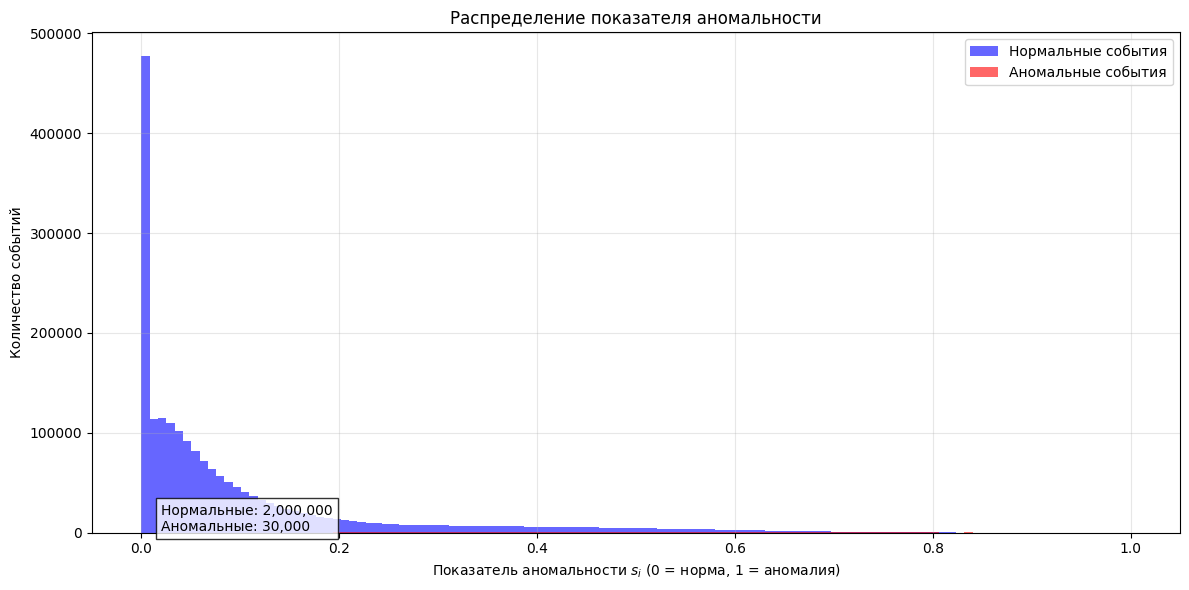
\includegraphics[scale=0.5]{inc/images/score_distribution}
    \caption{Распределение показателя аномальности $s_i$ для нормальных и аномальных трасс}
    \label{fig:score_distribution}
\end{figure}

Полученные результаты показывают, что нормальные и аномальные последовательности формируют различимые распределения значений $s_i$, что подтверждает применимость последовательностного логового подхода для обнаружения аномалий в системных логах и демонстрирует его работоспособность на реальных данных.